

\documentclass[12pt]{article}
\usepackage{comment}
\usepackage[utf8]{inputenc}
\usepackage[spanish]{babel}
\usepackage{amsmath}
\usepackage{makecell}
\usepackage{array}
\usepackage{graphicx}
\usepackage{geometry}
\usepackage{hyperref}
\bibliographystyle{IEEEtran}
\geometry{margin=2.5cm}




% Definir columna P que centra verticalmente y añade padding vertical extra
\newcolumntype{P}[1]{>{\centering\arraybackslash}m{#1}}
\newcommand{\mystrut}{\rule{0pt}{3.5ex}} % aumenta altura mínima fila




\begin{comment}
\title{Reporte Técnico: \\ Aspectos Dinámicos y Térmicos Clave en el Diseño de Secadores Solares de Café}
\author{Atilio Rodríguez \\ Proyecto de Investigación Etapa 1 de 2}
\date{Mayo 2025}    
\end{comment}

\usepackage{graphicx} % Para scalebox, asegúrate que esté cargado

\title{%
\vspace{2em}
{\scalebox{2}{\textbf{\textsc{REPORTE TÉCNICO}}}} \\[1.2em]
{\Large\bfseries Aspectos Dinámicos y Térmicos Clave en el Diseño de Secadores Solares de Café} \\[0.8em]
\rule{\textwidth}{9pt} \\[0.8em] 
{\large\itshape Dentro del marco del programa Nuevos Investigadores SENACYT, proyecto “Modelado y Diseño de Sistemas Inteligentes de Control de Temperatura y Humedad para Secadores Solares de Café en Panamá” (APY-NI-2024A-12)
}
}

\author{{\LARGE \textbf{Atilio A. Rodríguez Miranda}} \\[0.5em]
\large Proyecto de Investigación – Etapa 1 de 2}

\date{{\scshape Julio 2025}}


\begin{document}

\maketitle







\section{Resumen Ejecutivo}

Este informe técnico presenta una base conceptual  sobre los fundamentos térmicos, dinámicos y geométricos aplicables al diseño de secadores solares de café en climas tropicales, como parte de la primera etapa del proyecto “Modelado y Diseño de Sistemas Inteligentes de Control de Temperatura y Humedad para Secadores Solares de Café en Panamá” (APY-NI-2024A-12). A través de un enfoque sistemático, se identifican los parámetros críticos que afectan la eficiencia del secado, incluyendo geometría, distribución térmica, convección natural y condiciones climáticas exógenas, y se propone un marco analítico integral que servirá como base para el desarrollo de modelos numéricos avanzados, estrategias de control automático y validación experimental futura. Este estudio responde a la necesidad de mejorar la estandarización y eficiencia de los procesos de secado en la caficultura nacional, que optimicen la calidad del producto y aumenten la resiliencia de los pequeños productores frente a la variabilidad climática.


\clearpage

\section{Introducción}
\subsection{Contextualización del secado de café}

El secado de café en secadores solares es una técnica tradicional que ha perdurado en el tiempo, siendo muy valorada por su simplicidad y bajo costo. A pesar de ser una práctica extendida, su relevancia va mucho más allá de su historia, ya que el proceso de secado es fundamental para determinar la calidad final del café. Es en esta etapa donde se define si un café puede cumplir con los exigentes estándares internacionales que elevan su valor en el mercado, o si pierde calidad, lo que inevitablemente reduce las ganancias de los productores.\\

El éxito de este proceso depende del control de dos variables clave: la temperatura y la humedad. Estas condiciones deben mantenerse dentro de rangos específicos para asegurar que el café conserve su mejor perfil sensorial \cite{safri2021status}\cite{kudalkar2021smartdryer}. Un secado deficiente, ya sea por exceso o falta de control, puede dañar seriamente el grano, ya sea sobresecándolo y afectando sus atributos organolépticos, o dejándolo demasiado húmedo, lo que favorece el desarrollo de mohos y microorganismos perjudiciales.\\

\subsection{Problemática y limitaciones del método tradicional}


En Panamá, a pesar de contar con condiciones climáticas favorables para el cultivo de café y certificaciones de comercio justo y orgánico, la falta de automatización en el proceso de secado y la variabilidad de las condiciones climáticas presentan desafíos significativos. El uso predominante de métodos tradicionales de secado, que requieren una gran cantidad de mano de obra, limita la escalabilidad y eficiencia de la producción. Estos métodos no solo son intensivos en mano de obra, sino que también resultan en una calidad inconsistente debido a la falta de control sobre las condiciones ambientales variables, afectando negativamente la productividad y la capacidad de satisfacer una demanda creciente de cafés especiales.\\


Los secadores solares presentan ventajas importantes: son sostenibles porque no dependen de combustibles fósiles, son económicos porque no requieren equipos complejos, y contribuyen a mantener intactas las propiedades organolépticas del café, al no exponerlo a fuentes de calor que podrían alterar su sabor \cite{bradford2018drychain}\cite{srinivasan2021greenhouse}. Sin embargo, esta técnica tiene una gran limitación: está completamente a merced de las condiciones climáticas. Factores como la radiación solar, la humedad relativa y la temperatura del ambiente externo determinan el comportamiento interno del secador. En días nublados o húmedos, el proceso puede ser demasiado lento o incluso ineficaz, comprometiendo el producto final.\\

El secado a la intemperie continúa siendo una práctica tradicional ampliamente utilizada por pequeños productores de café debido a su bajo costo de implementación. Sin embargo, esta técnica presenta limitaciones inherentes relacionadas con la dependencia de condiciones climáticas favorables, la prolongada duración del proceso y la dificultad para garantizar una deshidratación uniforme y segura del grano.\\

El secado a la interperie del cafe supone las siguientes desventajas:

\begin{itemize}
    \item Toma mucho tiempo.
    \item Requiere de buenas condiciones climaticas.
    \item Los granos tienen que ser movidos constamente para condiciones homogeneas de secado. 
    \item Deben ser almacenados todas las noches para evitar el rocio mañanero. 
    \item El productor debe esperar a que el plot se calentado por el sol durante las mañanas. 
\end{itemize}


\subsection{Justificación del análisis técnico}

Mantener campos de temperatura y humedad uniformes en un secador solar de café es esencial para lograr un secado consistente y optimizar el control del proceso. La uniformidad en estas condiciones permite que todos los granos alcancen simultáneamente el contenido de humedad deseado, evitando variaciones que pueden afectar negativamente la calidad del café. Un sistema de secado predecible y controlado facilita la monitorización y ajuste del proceso, lo que no solo mejora la eficiencia y reduce la necesidad de intervención manual, sino que también asegura que se mantengan las propiedades sensoriales del café, contribuyendo así a un producto final de alta calidad.\\


En Perú, un plan piloto de producción de café honey gourmet (arábigo natural) desarrollado en la región de Satipo, Junín, alcanzó un precio estimado de venta de 330 dólares por quintal, generando un Valor Actual Neto (VAN) de aproximadamente S/.54.771 y una Tasa Interna de Retorno (TIR) del 66.5\%, lo que evidencia el alto potencial económico y la competitividad de este tipo de café en mercados especializados. Un aspecto crítico en el secado del café Honey en Perú es la falta de protocolos estandarizados  \cite{Alomia2021}. Los productores no cuentan con normas definidas, lo que impacta negativamente en la calidad sensorial del café. El proceso de secado, que se realiza de manera convencional aprovechando los rayos solares, está afectado por la variabilidad en la radiación solar diaria. Además, el tiempo de secado varía según la altitud: en áreas de menor altitud (800-1100 msnm), el secado del grano es más rápido (entre 8 a 12 días), mientras que en áreas de mayor altitud (más de 1100 msnm) el secado es más prolongado (más de 12 días), resultando en granos con mayor consistencia y densidad. Este contexto destaca la necesidad de estandarizar el proceso de secado adaptado a cada nivel altitudinal para mejorar la calidad del café.\\

En el control de temperatura y humedad para el secado de café, es fundamental permitir al caficultor ajustar el proceso de secado según sus necesidades. Si el objetivo es un secado gradual, para conservar las propiedades organolépticas del café, y el sistema de control no garantiza la estabilidad adecuada en el punto de referencia de temperatura y humedad, el control no cumpliría su propósito. Por tanto, el sistema debe optimizar el tiempo de respuesta y aplicar estrategias de control que sean ecológicas y económicas.\\

\clearpage



Lo que diferencia a esta investigación de otras realizadas en el mismo campo es su enfoque sistemático para abordar el problema. A diferencia de estudios anteriores, aquí se pretende definir de manera rigurosa todos los parámetros, condiciones, acciones de control y variables que interactúan durante la operación de un secador solar de café. Este enfoque integral no solo busca entender las relaciones entre estas variables, sino también establecer una base sólida para el diseño eficiente de sistemas de control de temperatura y humedad.\\



\subsection{Objetivo específico y alcance}


El objetivo es proporcionar una referencia técnica que sirva como punto de partida para futuros desarrollos en este campo. Más allá de optimizar el proceso de secado, se aspira a crear un marco normativo, una guía que responda a la creciente necesidad de estandarización en la industria del café, un aspecto que ha sido muy demandado por expertos y profesionales del sector.\\


Este autor aborda el problema de investigación a través de la siguiente teoría: \textit{El desempeño y la eficiencia de un secador solar de café están determinados por la interacción dinámica y sistémica de parámetros de diseño, condiciones iniciales de operación, variables de estado y acciones de control, cuya coherencia asegura la transferencia óptima de calor y masa durante el proceso de secado.}.\\




\section{Parámetros Clave de Diseño}
\label{sec:parametros_clave_de_diseño}

Entre los parámetros, se distinguen los parámetros de planta, que corresponden a las características físicas y estructurales del secador, parámetros de diseño, y los parámetros exógenos, que incluyen factores externos como las condiciones climáticas y la radiación solar. Las condiciones abarcan tanto las condiciones iniciales, es decir, el estado del sistema al inicio del proceso de secado, como las condiciones de frontera, que delimitan el comportamiento del sistema en función de los factores externos. Las acciones de control comprenden todas las acciones que pueden ser reguladas o auto-reguladas, cuyo propósito es modificar o mantener un estado deseado dentro del secador solar de café. Estas acciones permiten ajustar el sistema frente a perturbaciones o cambios en las condiciones externas, asegurando un proceso de secado óptimo. Finalmente, las variables de interés son aquellas que se deben monitorear y ajustar durante la operación, como la temperatura y la humedad interna.\\


\subsection{Parámetros de planta}
Estos son los aspectos físicos que definen la estructura y configuración del secador solar. Entre ellos se encuentran los parámetros geométricos (dimensiones y forma del secador), los parámetros de los materiales utilizados en su construcción, los parámetros de cimentación, que garantizan la estabilidad del secador, los parámetros de abertura en las fronteras, que controlan la ventilación y circulación de aire, y los parámetros de posición, que determinan la orientación y ubicación del secador respecto a la irradiancia solar.\\

Por lo general, los parámetros de planta son estacionarios, es decir, no varían con el tiempo, dado que la constitución física del secador solar permanece invariable durante su operación.\\% Sin embargo, sería interesante explorar casos en los que al menos uno de estos parámetros pudiera variar, ya que esto podría influir en el rendimiento del secador.\\

\subsection{Parámetros exógenos}
Por otro lado, los parámetros exógenos incluyen factores externos como la irradiancia solar, la temperatura externa, la humedad del ambiente y los parámetros del viento (velocidad y dirección). Estos parámetros son altamente dinámicos, es decir, cambian constantemente a lo largo del tiempo, y representan el principal desafío en el control eficiente de las plantas de secado solar \cite{friedland2005control}, ya que su variabilidad puede impactar directamente en las condiciones internas del secador.\\

%El diseño debe considerar latitud, radiación solar, humedad relativa y temperatura ambiente. Se utilizan datos locales y se recomienda modelado transitorio.

\subsection{Condiciones iniciales y de frontera}
Entre las condiciones que afectan la operación del secador solar se encuentran las condiciones iniciales y las condiciones de frontera.\\

Las condiciones iniciales hacen referencia a la distribución inicial de temperatura y la distribución inicial de humedad dentro del secador solar. Estas distribuciones no siempre son uniformes, ya que dependen del estado del café y del entorno en el momento en que comienza el proceso de secado.\\

Por otro lado, las condiciones de frontera se refieren a los valores de temperatura y humedad que existen fuera de las fronteras superficiales del secador solar, es decir, en el entorno externo. Estas condiciones externas, altamente variables, influyen en el comportamiento del secador al interactuar con su interior a través de las aberturas y otros medios de intercambio de aire.\\

Es importante destacar la aparente redundancia que existe entre las condiciones de frontera (como la temperatura externa) y los parámetros exógenos (como la temperatura del medio). La temperatura de frontera del secador solar no es necesariamente independiente o predefinida en todos los contextos. De hecho, esta temperatura está influenciada por un conjunto de parámetros exógenos, que incluyen la irradiancia solar, la temperatura del aire y las condiciones del viento. Además, también se ve afectada por variables internas, como la temperatura interna del secador.\\

Por lo tanto, es crucial que la definición de la frontera sea cuidadosamente considerada según el caso específico que se esté analizando, ya que esta interacción compleja puede tener un impacto significativo en el rendimiento del secador solar.\\

\subsection{Variables de interés u observables}

Las variables de interés son aquellas que definen el estado actual del secador solar. Entre ellas se encuentran la temperatura y humedad (en la extensión del secador), que son fundamentales para evaluar el desempeño del secador. Además, pueden incluirse otras variables relevantes, como el tiempo de asentamiento, que indica el tiempo que el café ha estado expuesto a las condiciones de secado, y la carga térmica en el secador, que se refiere a la cantidad de energía térmica que se aporta al sistema.\\

Estas variables son esenciales para monitorear y optimizar el proceso de secado, ya que influyen directamente en la calidad final del café y en la eficiencia del sistema. Un control adecuado de estas variables permite ajustar las condiciones del secador de manera efectiva, asegurando resultados consistentes y de alta calidad.


%\subsection{Gap: Rangos óptimos para Panamá}


\section{Tipologías y Geometrías de Secadores}

La geometría de un secador solar constituye un factor determinante en su desempeño térmico, ya que define directamente la relación entre la superficie expuesta ($S$) y el volumen interno ($V$). Esta relación $S/V$ influye tanto en la capacidad de captación de la radiación solar como en la acumulación y disipación de energía térmica en el interior del sistema. Por ello, resulta imprescindible analizar configuraciones geométricas representativas, como estructuras prismáticas, parabólicas o híbridas, para comprender cómo su morfología condiciona el balance energético, la distribución de temperatura y, en última instancia, la eficiencia del proceso de secado.


\subsection{Clasificación de geometrías}

Las geometrías se clasifican en dos categorías principales: \textbf{geometrías de revolución} y \textbf{geometrías prismáticas}. Este análisis se enfoca en aquellas que, por su fácil construcción, son ampliamente empleadas en la industria cafetalera.  La geometría impacta en la distribución del flujo y la acumulación térmica.\\

\subsubsection{Geometrías de revolución}

Las geometrías de revolución, aplicadas para la implementación de secadores solares de café, se generan al rotar figuras planas como rectángulos, triángulos rectos, secciones parabólicas o semicirculos, alrededor de un eje, creando volúmenes cerrados. \\



\clearpage

Las geometrías de revolución se dividen en dos subtipos:




\begin{enumerate}
    \item \textbf{Revolución simple}: Implica la rotación directa de figuras básicas, como triángulos.
    \item \textbf{Revolución compuesta}: Se forma al combinar una revolución simple con un cilindro, eliminando la superficie común entre ambas formas. %Esta clasificación es crucial para el diseño eficiente de secadores solares de café tipo invernadero, optimizando tanto su estructura como su funcionalidad.
\end{enumerate}

En la figura \ref{fig:croquis_1}, se muestran los tres tipos de geometrías consideradas en esta sección. En el cuadro \ref{tab:geometria_secadores_uno}, se observan las expresiones para la obtención de las áreas S y los volúmenes V. Considérese que a es el radio de la base del secador, $\sigma_{ba}$ es la relación entre la altura máxima del secador y el radio a, mientras que $\phi$ es el ángulo de inclinación del techo. 

\begin{figure}[h!]
    \centering
    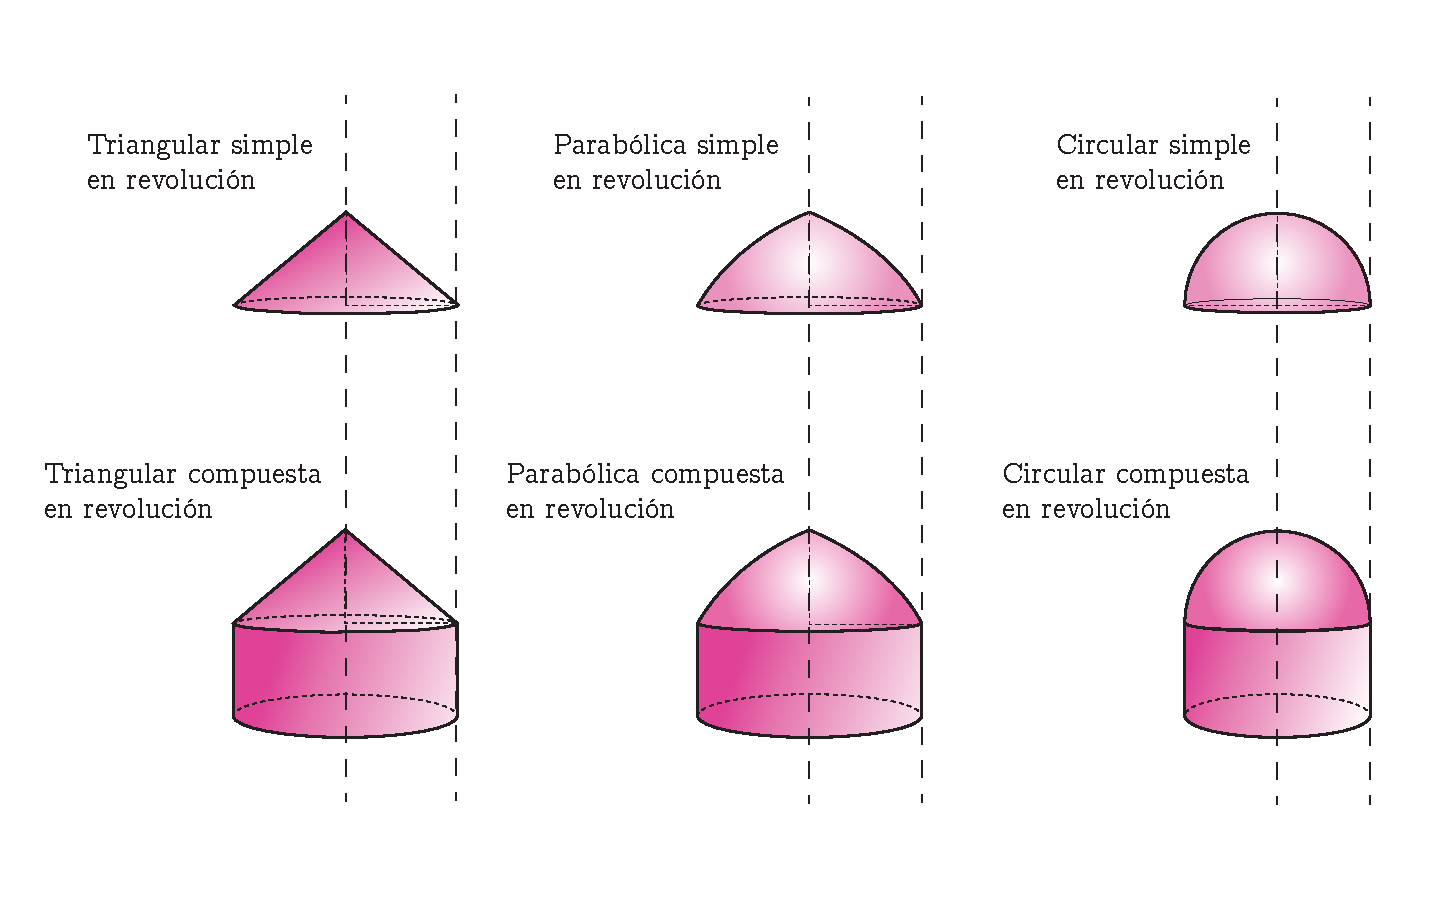
\includegraphics[width=0.75\textwidth]{croquis1.pdf}
    \caption{Geometrías de revolución comúnmente aplicadas para el diseño e implementación de secadores solares de café.}
    \label{fig:croquis_1}
\end{figure}

\begin{table}[h!]
\centering
\begin{center}
\begin{tabular}{|p{4cm}|p{6cm}|p{5cm}|}
\hline
\textbf{Geometría} & \textbf{$S$ (m$^2$)} & \textbf{$V$ (m$^3$)} \\
\hline
Triangular simple & 
$\pi a^2(\sigma_{ba}+1)$ &
$\frac{\pi}{3}a^3\sigma_{ba}$ \\
\hline
Triangular compuesta & 
$\pi a^2[2\sigma_{ba} - \tan\phi + 1]$ &
$\pi a^3\left(\sigma_{ba} - \frac{2}{3}\tan\phi\right)$ \\
\hline
Parabólica simple & 
$a^2\left[\frac{\pi}{6\sigma_{ba}}\Big((\sigma_{ba}^2+1)^{3/2}-1\Big)+\pi\right]$ &
$\frac{\pi}{2}\sigma_{ba}a^3$ \\
\hline
Parabólica compuesta & 
$\frac{a^2}{12\sigma_{ba}}\Big[(4\tan^2\phi+1)^{3/2}-1\Big] + \pi a^2[2\sigma_{ba} - 2\tan\phi + 1]$ &
$\pi a^3\left[1 - \frac{\tan\phi}{2}\right]$ \\
\hline
Circular simple & 
$3\pi a^2$ &
$\frac{2}{3}\pi a^3$ \\
\hline
Circular compuesta & 
$\pi a^2(3 + 2\sigma_{ba} - 2\tan\phi)$ &
$\pi a^3\Big(\frac{2}{3} + \sigma_{ba} - \tan\phi\Big)$ \\
\hline
\end{tabular}
\end{center}
\caption{Expresiones para la superficie $S$ y el volumen $V$ de secadores en revolución.}
\label{tab:geometria_secadores_uno}
\end{table}

 \clearpage

$$k\frac{\partial^2 u}{}$$

\subsubsection{Geometrías prismáticas}

Las geometrías prismáticas, utilizadas en la construcción de secadores solares de café, se obtienen mediante la extrusión de figuras planas como triángulos rectos, secciones parabólicas o semicircunferencias, a lo largo de una longitud determinada, generando volúmenes con sección transversal constante. Este enfoque permite diseñar configuraciones triangulares simples, parabólicas simples, circulares simples, así como variantes triangulares compuestas, parabólicas compuestas y circulares compuestas, optimizando la relación superficie/volumen para maximizar la captación solar y mejorar la eficiencia del secado.\\

En la figura \ref{fig:croquis_2}, se muestran los tres tipos de geometrías consideradas en esta sección.

\begin{figure}[h!]
    \centering
    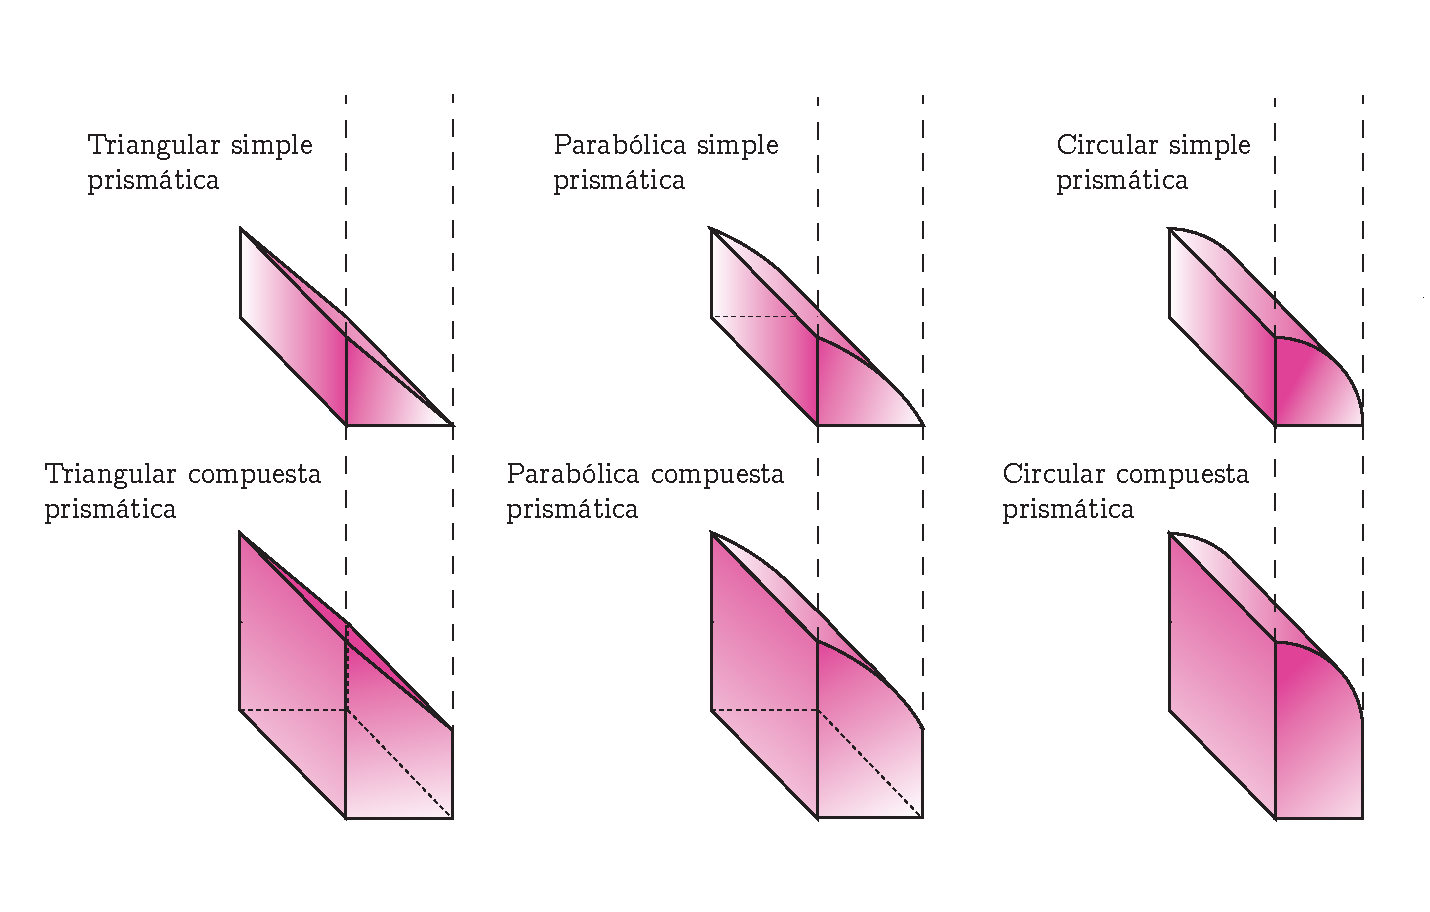
\includegraphics[width=0.80\textwidth]{croquis2.pdf}
    \caption{Geometrías prismáticas comúnmente aplicadas para el diseño e implementación de secadores solares de café.}
    %\caption{Transitorios para ambos secadores solares.}
    \label{fig:croquis_2}
\end{figure}

Se originan al extruir una figura plana a lo largo de una generatriz, resultando en volúmenes cerrados. Se clasifican en tres tipos:

\begin{enumerate}
    \item \textbf{Prismáticas simples}: Resultan de la extrusión de una figura geométrica básica.
    \item \textbf{Prismáticas compuestas}: Se obtienen al extruir la combinación de una figura geométrica simple con un rectángulo que tiene el mismo ancho que la base de dicha figura.
    \item \textbf{Prismáticas reflejas}: Se generan al reflejar una geometría prismática compuesta a lo largo de un plano que corta la curva generatriz y es perpendicular a la base del secador.
\end{enumerate}

%\clearpage

 En el cuadro \ref{tab:geometria_prismatica}, se observan las expresiones para la obtención de las áreas S y los volúmenes V. Considérese que a es la longitud de la base del secador, $\sigma_{ba}$ es la relación entre la altura máxima del secador y el radio a, mientras que $\phi$ es el ángulo de inclinación del techo. 


\begin{table}[h!]
\centering
\begin{tabular}{|p{4cm}|p{7cm}|p{5cm}|}
\hline
\textbf{Geometría} & \textbf{$S$ (m$^2$)} & \textbf{$V$ (m$^3$)} \\
\hline
Triangular simple prismática &
\vspace{0.001cm}
\(
\begin{aligned}
& \sigma_{ba}a^2 + (\sigma_{ba} + \sqrt{\sigma_{ba}^2+1} + 1)al
\end{aligned}
\) &
\vspace{0.001cm}
$\frac{1}{2}\sigma_{ba}a^2l$ \\
\hline

Triangular compuesta prismática &
\(
\begin{aligned}
& (2\sigma_{ba} + 1 - \tan\phi + \sec\phi)al \\
& + (2\sigma_{ba} - \tan\phi)a^2
\end{aligned}
\) &
$\frac{1}{2}(2\sigma_{ba} - \tan\phi)a^2l$ \\
\hline

Circular simple prismática &
\(
\begin{aligned}
& \left(\frac{\pi}{2}+2\right)al + \frac{\pi}{2}a^2
\end{aligned}
\) &
$\frac{\pi}{4}a^2l$ \\
\hline

Circular compuesta prismática &
\(
\begin{aligned}
& \Big(\frac{\pi}{2}+2+2\sigma_{ba} - 2\tan\phi\Big)al \\
& + \Big(\frac{\pi}{2} + 2\sigma_{ba} - \tan\phi\Big)a^2
\end{aligned}
\) &
$\Big(\frac{\pi}{2} + \sigma_{ba} - \tan\phi\Big)a^2l$ \\
\hline

Parabólica simple prismática &
\(
\begin{aligned}
& \Bigg( \frac{\sqrt{1+4\sigma_{ba}^2}}{2} + \frac{\ln(\sqrt{1+4\sigma_{ba}^2}+2\sigma_{ba})}{4\sigma_{ba}} \\
& + 1 + \sigma_{ba} \Bigg) al + \frac{4}{3}\sigma_{ba}a^2
\end{aligned}
\) &
$\frac{2}{3}\sigma_{ba}^2l$ \\
\hline

Parabólica compuesta prismática &
\(
\begin{aligned}
& \Bigg( \frac{\sqrt{1+4\tan^2\phi}}{2} \\&+\frac{\ln(\sqrt{1+4\tan^2\phi}+2\tan\phi)}{4\tan\phi} \\
& + 1 + 2\sigma_{ba} - \tan\phi \Bigg) al \\
& + 2a^2\Big(\frac{2}{3}\tan\phi + \sigma_{ba} - \tan\phi\Big)
\end{aligned}
\) &
$\Big(\frac{2}{3}\tan\phi + \sigma_{ba} - \tan\phi\Big)a^2l$ \\
\hline

\end{tabular}
\caption{Expresiones para la superficie $S$ y el volumen $V$ de secadores prismáticos}
\label{tab:geometria_prismatica}
\end{table}



\clearpage

En la figura \ref{fig:croquis3} se ilustran las configuraciones prismáticas reflejas consideradas para el análisis. Por su parte, en el cuadro \ref{tab:geometria_prismatica_simetrica} se presentan las expresiones analíticas correspondientes a la superficie expuesta ($S$) y al volumen interno ($V$) de cada una de estas geometrías, lo que permite evaluar comparativamente su capacidad de captación solar y almacenamiento térmico.


\begin{figure}[h!]
    \centering
    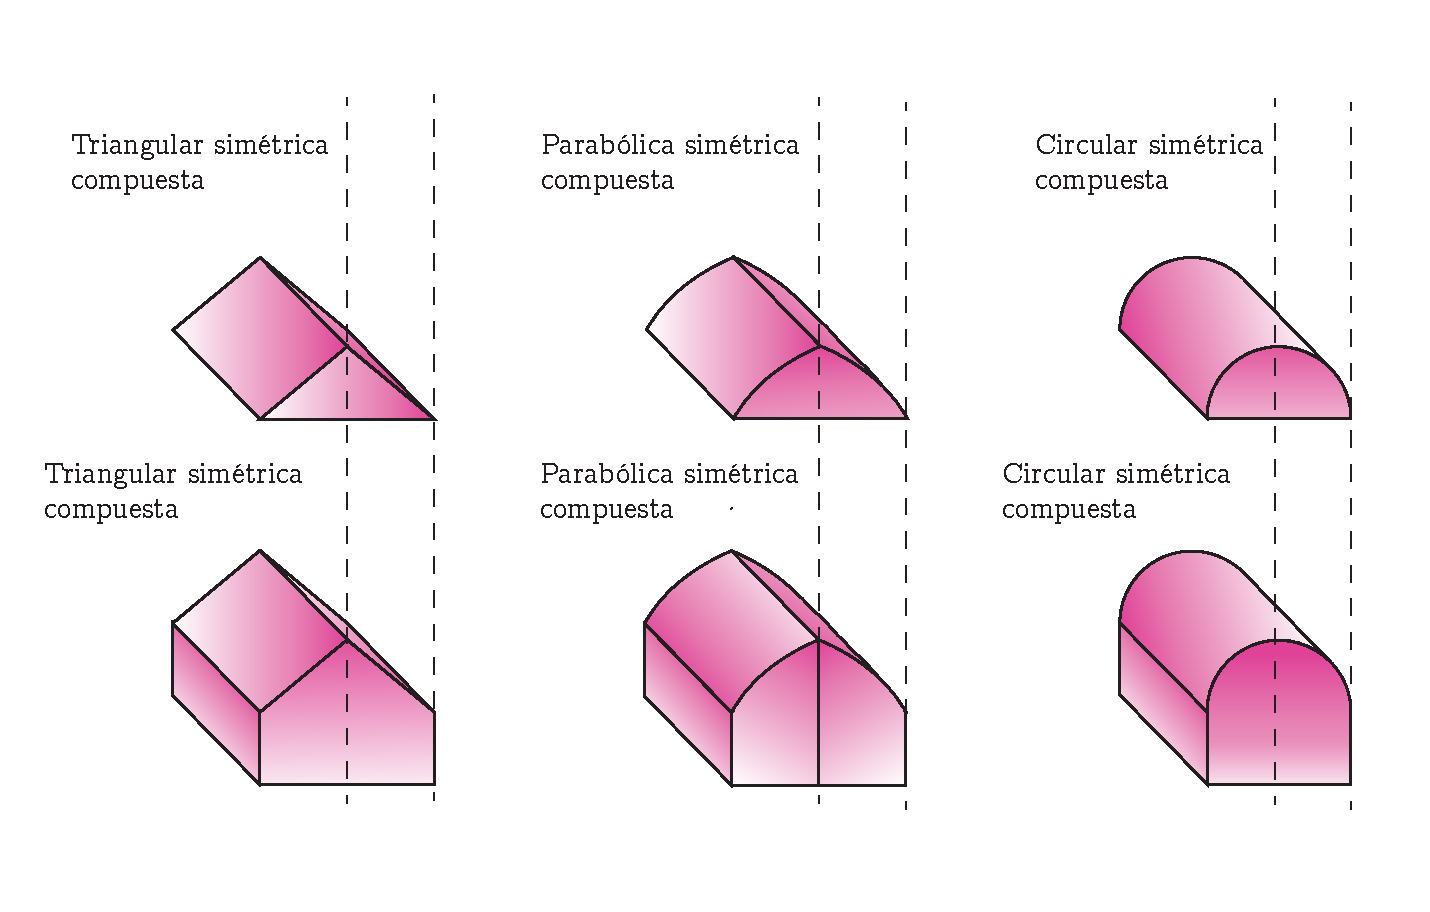
\includegraphics[width=0.80\textwidth]{croquis3.pdf}
    \caption{Geometrías prismáticas reflejas comúnmente aplicadas para el diseño e implementación de secadores solares de café.}
    %\caption{Transitorios para ambos secadores solares.}
    \label{fig:croquis3}
\end{figure}


\renewcommand{\arraystretch}{1.3} % más espacio entre filas

\begin{table}[h!]
\centering
\caption{Expresiones para la superficie $S$ y el volumen $V$ de secadores prismáticos simétricos}
\begin{tabular}{
    |p{4.2cm}|
    p{7cm}|
    p{4.5cm}|
    }
\hline
\textbf{Geometría} & \textbf{$S$ (m$^2$)} & \textbf{$V$ (m$^3$)} \\
\hline

Triangular simple simétrica prismática &
\parbox[t]{\hsize}{
$2(1+\sqrt{1+\sigma_{ba}^2})al + 2\sigma_{ba}a^2$
} &
$2\sigma_{ba}a^2l$ \\
\hline

Triangular compuesta simétrica prismática &
\parbox[t]{\hsize}{
$2(\sigma_{ba} + 1 - \tan\phi + \sec\phi)al$\\
$+ 2(\sigma_{ba} - \tan\phi)a^2$
} &
$(2\sigma_{ba} - \tan\phi)a^2l$ \\
\hline

Circular simple simétrica prismática &
\parbox[t]{\hsize}{
$\frac{\pi}{2}a^2l + \pi a^2$
} &
$\frac{\pi}{2}a^2l$ \\
\hline

Circular compuesta simétrica prismática &
\parbox[t]{\hsize}{
$\Big(\frac{\pi}{2} + 2 - 2\tan\phi\Big)al$\\
$+ \Big(\frac{\pi}{2} + 2\sigma_{ba} - \tan\phi\Big)a^2$
} &
$\Big(\frac{\pi}{4} + \sigma_{ba} - \frac{\tan\phi}{2}\Big)a^2l$ \\
\hline

Parabólica simple simétrica prismática &
\vspace{1mm}
\parbox[t]{\hsize}{
$\Big( \frac{\sqrt{1+4\sigma_{ba}^2}}{2} + \frac{\ln(\sqrt{1+4\sigma_{ba}^2}+2\sigma_{ba})}{4\sigma_{ba}} + 1 \Big)al$\\
$+ \frac{4}{3}\sigma_{ba}a^2$
} \vspace{1mm}&
$\frac{4}{3}\sigma_{ba}a^2l$ \\
\hline

\end{tabular}
\label{tab:geometria_prismatica_simetrica}
\end{table}





\clearpage




\subsection{Ventajas y limitaciones}
\label{subsec:ventajas_y_limitaciones}
%\section*{Síntesis del análisis matemático y físico de las geometrías}

El diseño de secadores solares para café requiere optimizar simultáneamente la superficie expuesta $S$ y el volumen interno $V$, dado que ambos parámetros condicionan la eficiencia de absorción de radiación y la capacitancia térmica del sistema. El área de superficie $S$ define la cantidad de radiación solar incidente que puede ser capturada, mientras que el volumen $V$ determina la capacidad del aire interior para almacenar calor y mantener la estabilidad térmica durante el proceso de secado. La relación $\frac{S}{V}$ emerge como una métrica fundamental para evaluar la eficiencia de transferencia de calor: idealmente debe ser alta para maximizar la captación de energía, pero sin reducir excesivamente el volumen, lo cual afectaría la homogenización de temperatura \cite{belessiotis2011solar}\cite{bradford2018drychain}
.\\

Las geometrías de revolución cúpulas parabólicas, semiesféricas o conos compuestos presentan expresiones de superficie y volumen que dependen no linealmente del radio $a$, la relación altura/base $\sigma_{ba}$ y el ángulo de inclinación $\tan\phi$. Por ejemplo, en la parabólica simple en revolución se tiene $S = \mathcal{O}(a^2)$ y $V = \mathcal{O}(a^3)$, resultando en $\frac{S}{V} \approx \mathcal{O}(1/a)$. Esto implica que para radios grandes, la relación $\frac{S}{V}$ disminuye, lo que reduce la tasa de pérdida térmica, pero a costa de limitar la absorción solar específica por unidad de volumen de aire. Las geometrías compuestas integran el parámetro $\tan\phi$ para modificar la inclinación de las paredes, incrementando la exposición solar y favoreciendo el flujo convectivo natural. La circular simple, con $S = 3\pi a^2$ y $V = \frac{2}{3}\pi a^3$, muestra una de las menores relaciones $\frac{S}{V}$, siendo idónea para retención de calor, aunque menos eficiente para extracción rápida de humedad.\\

Las geometrías prismáticas, definidas como extrusiones longitudinales de perfiles básicos, presentan una dependencia lineal de $S$ y $V$ respecto a la longitud $l$. Por ejemplo, en la triangular simple prismática: 
\[
S = \sigma_{ba}a^2 + (\sigma_{ba} + \sqrt{\sigma_{ba}^2+1} + 1)al,\quad V = \frac{1}{2}\sigma_{ba}a^2l.
\]
Para longitudes grandes, la relación $\frac{S}{V}$ se estabiliza como $\mathcal{O}(1/a)$, lo que ofrece mayor flexibilidad modular y control térmico estable. Además, las variantes compuestas ajustan $\tan\phi$ para inclinar paredes laterales, aumentando la captación solar y modulando la convección natural interna. Este diseño permite alcanzar ángulos críticos de reflexión más amplios, optimizando la captación solar durante más horas del día.\\

Las geometrías prismáticas simétricas duplican secciones y planos inclinados para habilitar flujos de aire bidireccionales. Por ejemplo, en la parabólica simple prismática simétrica se observa que:
\[
S \approx 2 \times S_{\text{parabólica simple prismática}}, \quad V \approx 2 \times V_{\text{parabólica simple prismática}},
\]
manteniendo la relación $\frac{S}{V}$ similar pero mejorando significativamente la ventilación cruzada. Este atributo es valioso para secadores de alta carga, donde la eliminación de zonas frías y la homogeneidad térmica son cruciales.\\

De forma transversal, se identifican factores clave para la optimización geométrica:
\begin{itemize}
    \item En zonas de alta radiación difusa, las geometrías parabólicas compuestas son ideales, ya que su superficie $S$ se incrementa con términos cúbicos en $\tan\phi$, maximizando la exposición solar.
    \item Para secadores modulares y de construcción sencilla, las formas prismáticas (simples o compuestas) son preferibles, pues permiten mantener un $\frac{S}{V}$ elevado con láminas planas, facilitando la manufactura y el montaje.
    \item Para retención térmica nocturna, la geometría circular simple en revolución destaca por su baja relación $\frac{S}{V}$, minimizando pérdidas de calor \cite{mustayen2014performance}.
    \item Las configuraciones prismáticas simétricas permiten cámaras internas con flujo cruzado, mejorando la eficiencia de secado y evitando acumulación de humedad.
\end{itemize}

Finalmente, cabe destacar la riqueza matemática de expresiones como $\ln(\sqrt{1+4\sigma_{ba}^2}+2\sigma_{ba})$ en las geometrías parabólicas, que muestra cómo la curva parabólica optimiza la relación entre área y longitud, manteniendo un equilibrio entre captación y retención de calor. La selección adecuada de $a$, $\sigma_{ba}$ y $\tan\phi$ se torna esencial para dimensionar secadores solares que maximicen la captación diurna y minimicen pérdidas nocturnas \cite{belessiotis2011solar}\cite{mustayen2014performance}, adaptándose a las condiciones climáticas locales y a la escala de producción.

\clearpage

\subsection{Cuadro comparativo de eficiencia}

A continuación, se presenta una tabla comparativa que sintetiza las principales características geométricas y térmicas de las configuraciones de secadores solares analizadas. Este compendio resulta del análisis matemático detallado efectuado en la sección \ref{subsec:ventajas_y_limitaciones}, donde se evaluaron ventajas y limitaciones de cada diseño en función de criterios clave como la facilidad de fabricación, relación superficie-volumen, dinámica del flujo de aire, inclinación solar, capacitancia térmica y eficiencia en la captación solar. Esta comparación permite identificar las configuraciones más adecuadas para optimizar el proceso de secado, considerando tanto aspectos constructivos como térmicos.

\renewcommand{\arraystretch}{1.2}
\setlength{\tabcolsep}{6pt}

\begin{table}[h!]
\centering
\begin{tabular}{|P{4.5cm}|P{3.3cm}|P{3.3cm}|P{3.7cm}|}
\hline
\textbf{Aspecto} & \textbf{Revolución} & \textbf{Prismática} & \textbf{Prismática Simétrica} \\
\hline

Facilidad de fabricación &
\mystrut \makecell[c]{\textbf{\textsc{Compleja}} \\ (formas curvas)} &
\mystrut \makecell[c]{\textbf{\textsc{Sencilla}} \\ (paneles planos)} &
\mystrut \makecell[c]{\textbf{\textsc{Moderada}} \\ (paneles duplicados)} \\
\hline

Relación S/V &
\mystrut Depende fuertemente de $a$; decrece para radios grandes &
\mystrut Depende linealmente de $l$; ajustable modularmente &
\mystrut Similar, con mejor distribución térmica \\
\hline

Flujo de aire &
\mystrut Natural centrado &
\mystrut Direccional canalizado &
\mystrut Bidireccional; ventilación cruzada \\
\hline

Ángulo de inclinación ($\tan\phi$) &
\mystrut Clave para reflejo solar y convección pasiva &
\mystrut Ajusta exposición solar lateral &
\mystrut Permite mayor homogeneidad térmica \\
\hline

Capacitancia térmica &
\mystrut {\textbf{\textsc{Alta}}; volúmenes cerrados retienen calor} &
\mystrut {\textbf{\textsc{Moderada}}; modular} &
\mystrut {\textbf{\textsc{Alta}}; adecuada para cargas variables} \\
\hline

Eficiencia solar &
\mystrut {\textbf{\textsc{Alta}} con radiación incidente baja} &
\mystrut {\textbf{\textsc{Alta}} para secado pasivo lineal} &
\mystrut {\textbf{\textsc{Óptima}} para carga variable y clima inestable} \\
\hline
\end{tabular}
\caption{Comparación de las principales características geométricas y térmicas de diferentes configuraciones de secadores solares de café, destacando sus ventajas en términos de fabricación, eficiencia energética, flujo de aire y capacidad térmica.}
\label{tab:comparativa_geometrias}
\end{table}


\clearpage




%\subsection{Gap: Métricas de referencia}


\section{Fundamentos Físicos y Dinámicos}

El aire dentro del secador es calentado por el sol, lo que reduce su humedad relativa. Este aire caliente y seco circula alrededor de los granos de café húmedos, absorbiendo el agua y secándolos gradualmente. La circulación del aire se mantiene debido a la diferencia de temperatura entre el interior y el exterior del secador: el aire caliente asciende y sale por las aberturas cercanas al techo, mientras que el aire frío entra a través de las aberturas cercanas al suelo, creando un flujo continuo.\\

En la figura~\ref{fig:diagrama_trx} se observan los distintos mecanismos de transferencia de calor que tienen lugar en la sección transversal del recubrimiento de un secador solar de café. Se distinguen los procesos de transferencia por radiación, convección y conducción, así como el calor absorbido directamente como resultado de la radiación solar incidente sobre la superficie.


\begin{figure}[h!]
    \centering
    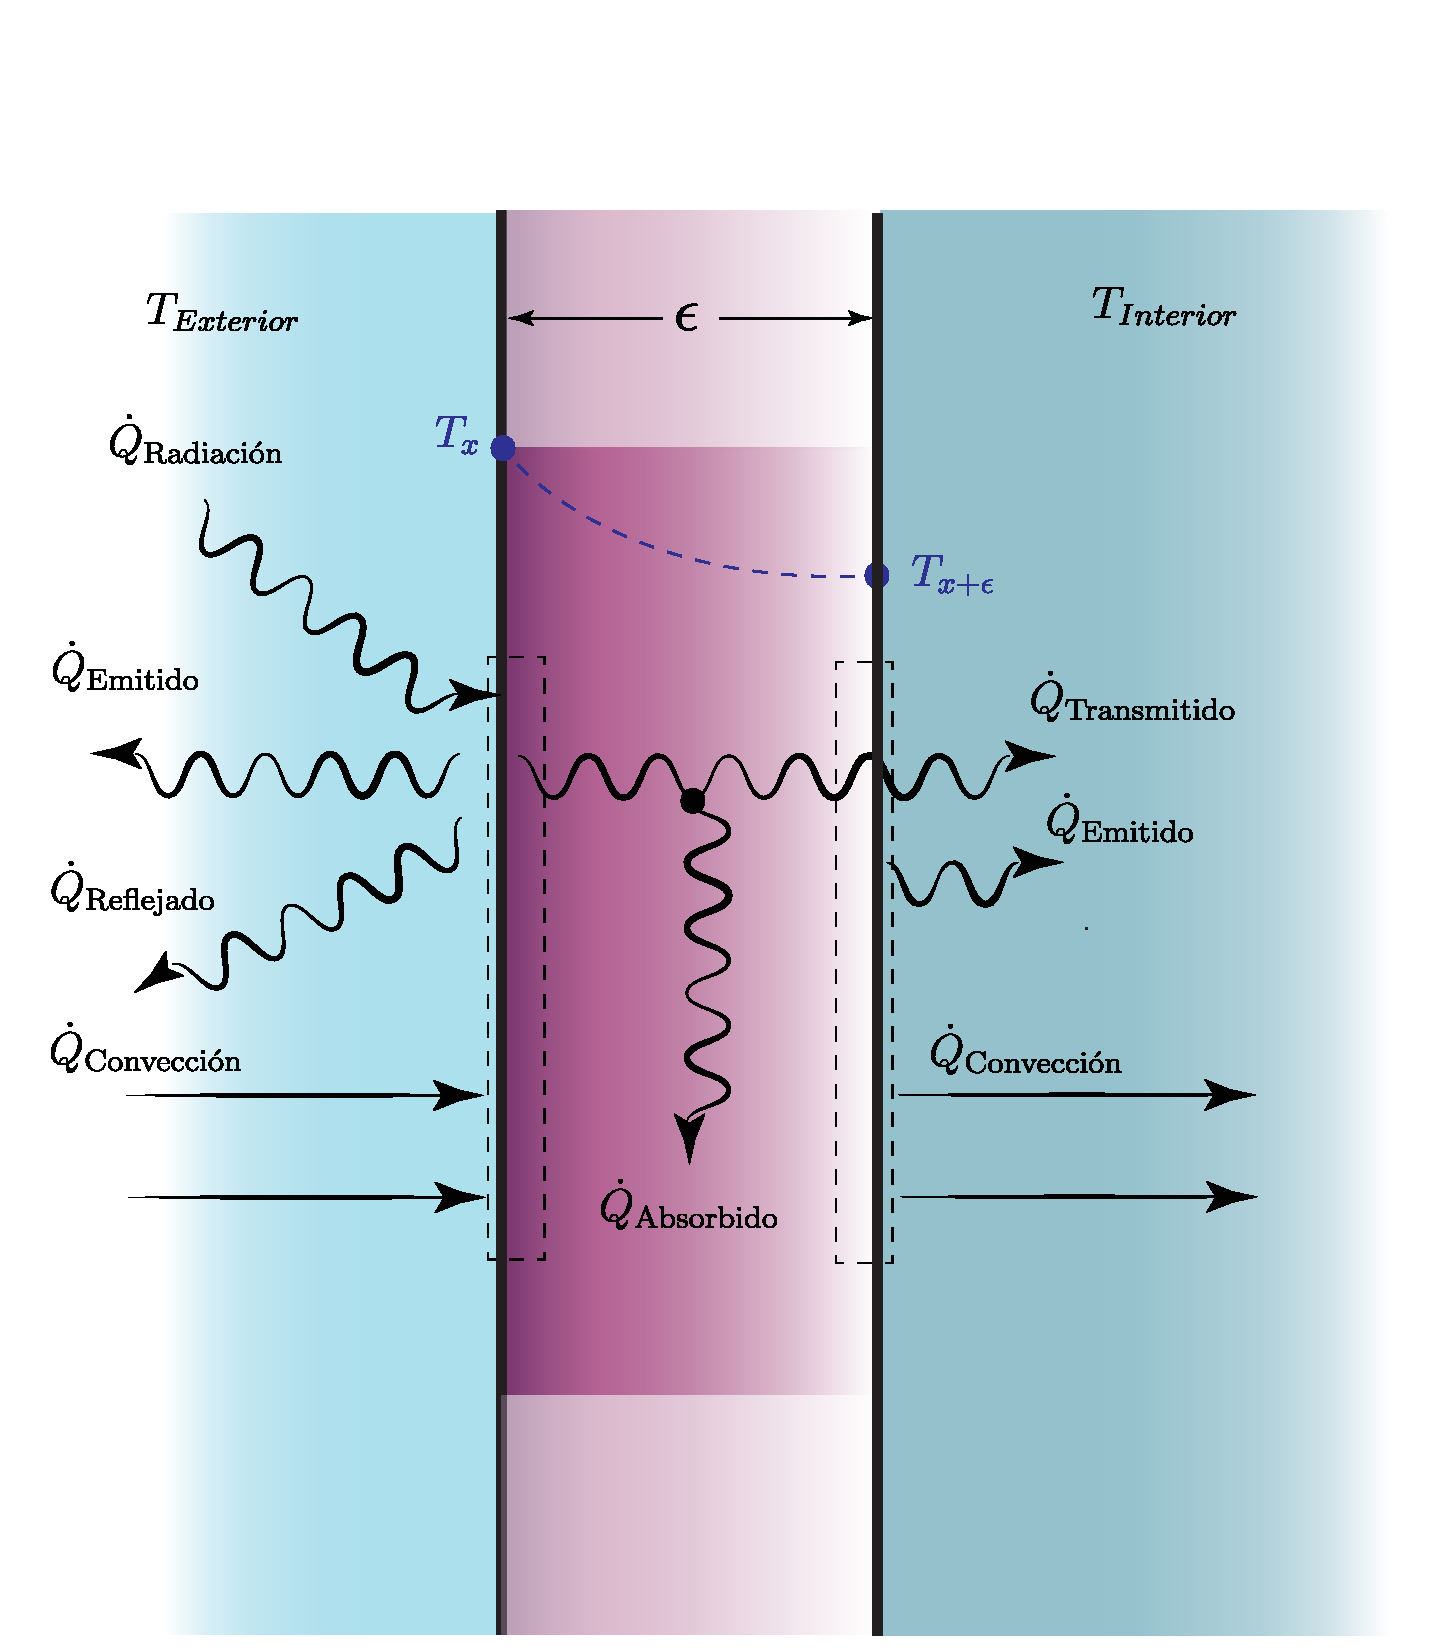
\includegraphics[width=0.50\textwidth]{transferencia.eps}
    \caption{Transferencia de calor en un elemento de volumen de la sección transversal del recubrimiento de un secador solar. A la izquierda se tiene el aire exterior, mientras que a la derecha, se tiene el aire interior del secador solar. }
    \label{fig:diagrama_trx}
\end{figure}



\begin{itemize}
  \item \textbf{Transferencia de calor:} convección natural y forzada, conducción, radiación directa, difusa y reflejada.
  \item \textbf{Transferencia de masa:} evaporación de humedad desde el grano al aire caliente.
  \item \textbf{Buoyancia:} movimiento inducido por gradientes térmicos.
  \item \textbf{Turbulencia:} modelada según el régimen de flujo (RANS, $\kappa$--$\varepsilon$).
\end{itemize}


\subsection{Transferencia de calor y masa}

Con el fin de abordar los mecanismos de transferencia de calor de un secador solar de café arbitrario, se comienza con un análisis teórico de la distribución de temperaturas en estado estacionario. Considerando que en estado estacionario no hay acumulaciòn de calor, ni variación de los parámetros internos y exógenos, se establecen los siguientes supuestos:

\begin{enumerate}
    \item No hay generaciòn de calor en ningùn punto sobre o dentro de las fronteras del secador solar. 
    \item No hay flujos de aire desde, o hacìa, el secador solar. 
    \item La temperatura del medio es constante en toda su extensiòn.
    \item La irrandiancia solar media en el ambiente es constante en las vecindades del secador solar. 
    \item No hay transferencia de calor en la base del secador solar, esto es, la base del secador solar està aìslada. 
\end{enumerate}

El balance de transferencia de calor en la superficie del secador solar considera la igualdad entre los flujos térmicos entrantes y salientes, integrando los mecanismos de radiación, convección y conducción. Al discretizarse la superficie, este balance se expresa como una suma de contribuciones locales que reflejan la absorción de radiación solar, pérdidas convectivas y emisiones radiativas. Para determinar la distribución de temperaturas en estado estacionario es necesario conocer la tasa de transferencia de calor en cada punto de la superficie y las condiciones térmicas en la interfaz aislante-aire interno, permitiendo así un modelado preciso del comportamiento térmico del sistema.\\

Considerando que:

\begin{itemize}
    \item $\vec{q}_i$: Vector flujo de calor entrante a la superficie.
    \item $\vec{q}_o$: Vector flujo de calor saliente desde la superficie.
    \item $\vec{dA}_n$: Vector área diferencial de la superficie, orientado normalmente.
    \item $I_o$: Intensidad de radiación solar incidente sobre la superficie.
    \item $\hat{r}(n)$: Vector unitario en la dirección de incidencia de la radiación en el elemento $n$.
    \item $\alpha$: Coeficiente de absorción de la superficie.
    \item $Tr$: Transmitancia del material del recubrimiento.
    \item $h(n)$: Coeficiente convectivo local en el elemento $n$.
    \item $T_s(n)$: Temperatura superficial en el elemento $n$.
    \item $T_\infty$: Temperatura ambiente del aire circundante.
    \item $\epsilon$: Emisividad del recubrimiento.
    \item $\sigma$: Constante de Stefan-Boltzmann.
\end{itemize}




$$\oint \vec{q}_i\cdot \vec{dA}_n = \oint \vec{q}_e\cdot\vec{dA}_n$$

$$\oint[\vec{q}_i-\vec{q}_o]\cdot\vec{dA}_n = 0$$

$$\oint[I_o\hat{r}(n)(\alpha+Tr)-h(n)(T_s(n)-T_\infty)\hat{n}-\epsilon\sigma(T_s^4(n)-T_\infty^4)\hat{n}]\cdot\vec{dA}_n = 0$$

Si consideramos elementos finitos, discretizando $dA_n \approx \Delta A_n$, y asumiendo $\Delta A_n$ constante:

$$\Sigma_n [I_o(\alpha+Tr)\cos(\theta)-h(n)(T_s(n)-T_\infty)-\epsilon\sigma(T_s^4(n)-T_\infty^4)] = 0$$

La ecuación refleja el equilibrio dinámico entre la energía solar absorbida y las pérdidas térmicas por convección y radiación en la superficie del secador, mostrando que la eficiencia térmica depende críticamente de la orientación, la geometría y las propiedades ópticas del material (absorción, transmitancia y emisividad). Además, evidencia cómo las condiciones ambientales y la diferencia entre la temperatura superficial y la ambiental impactan directamente la capacidad de mantener temperaturas óptimas para el secado, resaltando la necesidad de un diseño cuidadoso y estrategias de control térmico para maximizar el rendimiento del sistema.


\subsection{Buoyancia y flujo de aire}
\label{subsec:buoyancia_y_flujo_de_aire}
El análisis del flujo de aire en el secador solar requiere la consideración de la fuerza de flotación térmica, la cual influye directamente en el movimiento convectivo dentro del sistema. Para ello, se parte de la ecuación de momento vertical de Navier-Stokes, adaptada para flujos estables y con variaciones de densidad inducidas por diferencias de temperatura.\\

La ecuación de momento, de Navier Stokes \cite{incropera_heatmass_2007}, en el vertical se muestra en la ecuación \ref{eqn:stokes_buoyancia}:

\begin{equation}
\label{eqn:stokes_buoyancia}
    u\frac{\partial u}{\partial x}+v\frac{\partial u}{\partial y} = -\frac{1}{\rho}\frac{dp_\infty}{dx}-g+v\frac{\partial^2u}{\partial y^2}
\end{equation}

Considerando un flujo estable, prácticamente en reposo, la ecuación \ref{eqn:stokes_buoyancia} queda como:

$$\frac{dp_\infty}{dx} = -\rho_\infty g$$

Sustituyendo nuevamente en la ecuación \ref{eqn:stokes_buoyancia}, y estableciendo un régimen estable:

\begin{equation}
\label{eqn:capa_limite}
    u\frac{\partial u}{\partial x}+v\frac{\partial u}{\partial y} = -g\frac{\Delta\rho}{\rho}+v\frac{\partial^2u}{\partial y^2}
\end{equation}


La ecuación \ref{eqn:capa_limite}, ha de cumplirse sobre todo punto de la capa límite de convección libre. Si las variaciones de densidad son únicamente debidas a variaciones de temperatura, el término $g\frac{\Delta\rho}{\rho}$, está asociado con una propiedad del fluido (en este caso aire), conocida como \textbf{coeficiente de expansión volumétrica} (véase la ecuación \ref{eqn:expansion_volumetrica}):

\begin{equation}
\label{eqn:expansion_volumetrica}
    \beta = -\frac{1}{\rho}\left(\frac{\partial\rho}{\partial T}\right)_p
\end{equation}



Considerando que: 


$$\beta \approx -\frac{1}{\rho}\frac{\Delta\rho}{\Delta T} = -\frac{1}{\rho}\frac{\rho_\infty-\rho}{T_\infty-T}$$

Se tiene que.

$$(\rho_\infty-\rho)\approx\rho\beta(T-T_\infty)$$

Esta simplifación corresponde a la \textsc{\textbf{Aproximación de Boussinesq}}. Sustituyendo en \ref{eqn:capa_limite}, se obtiene la ecuación \ref{eqn:stokes-boussinesq}:

\begin{equation}
\label{eqn:stokes-boussinesq}
    u\frac{\partial u}{\partial x}+v\frac{\partial u}{\partial y} = g\beta(T-T_\infty)+v\frac{\partial^2u}{\partial v^2}
\end{equation}

En este punto es evidente que la fuerza de buoyancia gobierna los patrones de flujo del aire confinado dentro del secador solar. Esta fuerza es una medida de la diferencia entre la temperatura promedio y la temperatura máxima en una región dada, así como de la propiedad de expansión volumétrica del aire. \\


En la configuración de un secador solar de café, la base del secador ($T_\text{base}$) y el recubrimiento superior ($T_\text{top}$) definen un gradiente térmico vertical que determina el sentido de la fuerza de flotación:\\

\begin{itemize}
    \item \textbf{Caso 1: $T_\text{recubrimiento} < T_\text{base}$.}  
    En este escenario, la temperatura decrece con la altura, por lo que la fuerza de flotación $g\beta(T - T_\infty)$ es positiva en la capa de aire adyacente a la base. Esto genera un movimiento ascendente del aire caliente, que se traduce en la formación de células de convección natural dentro de la cavidad del secador. La circulación resultante tiende a ser inestable y puede inducir una mezcla más eficiente, favoreciendo el transporte de calor y masa hacia el producto.
    
    \item \textbf{Caso 2: $T_\text{recubrimiento} > T_\text{base}$.}  
    En este caso inverso, el aire adyacente al recubrimiento superior es más caliente que la base. Dado que la flotación térmica depende de la diferencia $T-T_\infty$, el signo de la fuerza de flotación se invierte, pero su efecto neto se ve contrarrestado por la geometría física del techo que restringe el flujo ascendente. Esto provoca una estratificación estable, anulando la circulación convectiva. El resultado es la formación de capas de aire de diferente temperatura que dificultan la renovación del aire húmedo y reducen la eficiencia del secado.
\end{itemize}




\begin{figure}[h!]
    \centering
    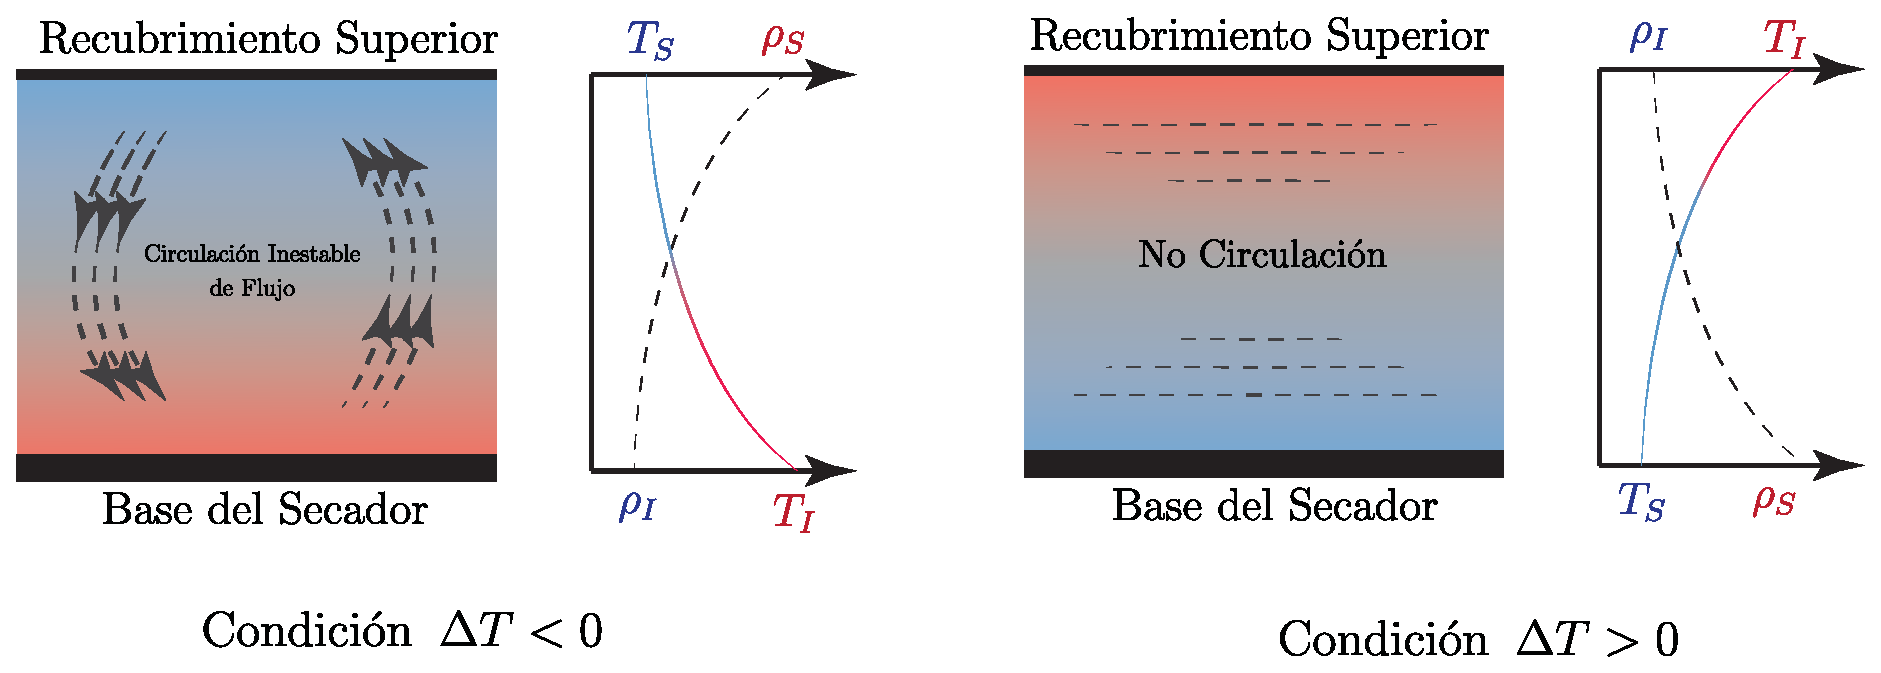
\includegraphics[width=0.99\textwidth]{diagrama_buoyancia.eps}
    \caption{Condiciones de diferencia de temperatura entre el recubrimiento superior y la base de un secador solar de café. Si la temperatura del recubrimiento superiror es mayor a la de la base, se inducirá una circulación inestable de flujo, de lo contrario, no habrá circulación de aire dentro del secador.  }
    \label{fig:diagrama_buoyancia}
\end{figure}

\noindent
De este análisis se desprende que el diseño geométrico y el manejo de materiales de recubrimiento deben buscar condiciones que mantengan $T_\text{recubrimiento} > T_\text{top}$ para aprovechar la fuerza de flotación. La ecuación de Stokes-Boussinesq muestra que el gradiente térmico es el factor determinante para inducir un flujo natural continuo, minimizando la necesidad de ventilación forzada.\\

Finalmente, cabe destacar que la magnitud del término de difusión viscosa, $\nu\frac{\partial^2 u}{\partial y^2}$, actúa como freno disipativo de la velocidad del flujo generado por la flotación. Por tanto, para secadores de gran altura o con recubrimientos con baja conductividad, el diseño debe equilibrar la generación de flotación y la disipación viscosa para mantener un patrón de circulación eficiente.



\subsection{Turbulencia y régimen de flujo}

El rendimiento de un secador solar de café depende profundamente del comportamiento del flujo de aire en su interior. La ecuación de momento bajo la aproximación de Boussinesq muestra que los patrones de flujo están dominados por la flotación térmica: las diferencias de temperatura generan fuerzas de cuerpo (buoyancia) que impulsan el movimiento natural del aire. En términos prácticos, la relación entre la temperatura de la base del secador y la del recubrimiento superior condiciona si se establecen células convectivas estables, inestables o si, por el contrario, se inhibe la circulación.\\

Cuando la temperatura del recubrimiento superior es mayor que la de la base, la flotación se vuelve estable: el aire caliente se encuentra confinado y la fuerza de flotación que debería impulsar el flujo es anulada por la resistencia del techo. Esto provoca que el flujo se mantenga en régimen laminar o incluso estratificado, lo cual reduce significativamente la mezcla de aire y la renovación de la humedad. Como consecuencia, aparecen zonas con alto contenido de humedad y el secado es más lento y menos uniforme.\\

En contraste, cuando la base del secador está a mayor temperatura que el recubrimiento, se crea una flotación inestable. Esta condición genera corrientes de aire ascendentes que fomentan la formación de células convectivas. A medida que se incrementa la diferencia de temperatura, la energía de flotación supera la disipación viscosa y surgen inestabilidades que pueden evolucionar hacia un régimen de flujo transicional o parcialmente turbulento. En este escenario, la turbulencia natural desempeña un papel positivo: mejora la mezcla de aire, rompe capas límite de humedad sobre la superficie del café y favorece una transferencia de calor más uniforme. \\

Este fenómeno es especialmente relevante para geometrías abiertas o prismáticas modulares, que permiten un desarrollo controlado de la convección. Por ejemplo, una geometría parabólica compuesta puede maximizar la captación solar y dirigir mejor el flujo, mientras que las formas prismáticas, al ser modulares, ofrecen un canal de flujo direccional que puede potenciar la ventilación natural sin requerir sistemas mecánicos adicionales.\\

Un punto clave es la relación entre área de superficie expuesta y volumen interno ($S/V$). Un $S/V$ alto favorece la captación de radiación y la transferencia de calor, pero también puede aumentar las pérdidas térmicas durante la noche. Por eso, la elección de la forma geométrica y los parámetros de diseño como la altura relativa ($\sigma_{ba}$) y el ángulo de inclinación ($\tan\phi$) se vuelven esenciales para ajustar la intensidad del flujo y su régimen dominante.\\

En síntesis, un secador solar de café bien diseñado debe propiciar gradientes térmicos que induzcan flotación inestable, manteniendo un flujo predominantemente transicional o suavemente turbulento para garantizar una renovación eficiente del aire y una eliminación homogénea de la humedad. Comprender cómo la flotación, la geometría y la turbulencia interactúan permite optimizar tanto la eficiencia energética como la calidad final del café, equilibrando la absorción solar diurna con una retención adecuada del calor durante la noche.



\subsection{Condiciones Climáticas}

La \textbf{climatología local} es un factor determinante en el diseño, operación y optimización de un secador solar de café, pues define los límites y oportunidades de aprovechamiento de la energía solar y la dinámica del flujo de aire.

\begin{enumerate}
    \item \textbf{Condiciones climáticas como parámetros exógenos} \\
    A diferencia de los parámetros geométricos o de operación interna (como forma, ángulo de inclinación o posición de ventilaciones), el clima es un \emph{parámetro exógeno}: no se puede controlar, pero sí se puede describir y predecir estadísticamente. Variables como la radiación solar incidente, la temperatura ambiente, la humedad relativa y la velocidad del viento determinan la energía disponible para el secado y la facilidad con la que se evacua la humedad.

    \item \textbf{Modelar la climatología para reducir incertidumbre} \\
    Conocer la climatología permite dimensionar el secador de forma realista. Por ejemplo, saber cuántas horas de sol directo se tienen por día, cuál es el rango de temperaturas y cómo varía la humedad relativa a lo largo del día y del año. Estos datos se integran en modelos de transferencia de calor y masa para prever la eficiencia de secado en escenarios promedio y extremos. Sin esta modelación, se corre el riesgo de sobre- o subdimensionar componentes clave (área colectora, aberturas de ventilación, materiales de recubrimiento) y, por ende, perder eficiencia.

    \item \textbf{Optimización pasiva del flujo y la energía} \\
    El conocimiento detallado de la climatología también facilita estrategias de diseño \emph{pasivas}, como orientar la estructura para maximizar la radiación solar, optimizar ángulos de inclinación de techos para captar mejor la radiación difusa en días nublados o ubicar aberturas de forma que aprovechen vientos predominantes y refuercen la ventilación natural.

    \item \textbf{Robustez frente a la variabilidad} \\
    Modelar las condiciones climáticas mediante parámetros exógenos aporta \emph{robustez}: permite simular múltiples escenarios (como temporadas especialmente húmedas) y anticipar estrategias de operación, como cerrar ciertas ventilas para conservar calor o abrirlas para evitar la condensación.

\end{enumerate}

\noindent En síntesis, entender la climatología y traducirla en parámetros exógenos no elimina la variabilidad climática, pero sí permite diseñar un sistema que se adapte a ella de forma eficiente, maximizando la captación solar, favoreciendo patrones de flujo deseables (convección natural, turbulencia controlada) y asegurando la calidad del café sin depender de fuentes de energía externas.


%\subsection{Gap recomendado: validación experimental}







\section{Acciones de Control y Estrategias de Optimización}

Las acciones de control son aquellas intervenciones realizadas por los actuadores instalados en el secador solar, con el propósito de preservar o modificar su estado actual. Estas acciones se enfocan en garantizar que las condiciones de temperatura y humedad dentro del secador se mantengan dentro de los rangos óptimos para su operación eficiente. Los actuadores responden a las variaciones tanto internas como externas, ajustando dinámicamente el sistema para que el proceso de secado del café sea consistente y controlado, independientemente de las fluctuaciones en las condiciones climáticas.\\


Los secadores mecánicos son dispositivos que permiten un control preciso y constante de las variables involucradas, por lo que el proceso de secado que generan es determinístico. En el caso del secado solar, se busca replicar, en la medida de lo posible, este comportamiento determinístico. Para lograrlo, es fundamental contar con un buen conocimiento de las variables meteorológicas, un diseño constructivo eficiente, y el apoyo de simulaciones y modelos matemáticos. De esta manera, se pretende hacer que el secado solar sea lo más predecible y eficiente posible.\\

\clearpage

\subsection{Mecanismos de control de temperatura y humedad}

El diseño de un sistema de secado solar de café con desempeño óptimo requiere no solo una geometría adecuada y estrategias pasivas de captación y retención de calor, sino también la integración de mecanismos de control automático que garanticen condiciones de temperatura y flujo de aire estables, incluso frente a fluctuaciones ambientales. Para ello, se propone un esquema de control en lazo cerrado que permite monitorear continuamente las variables críticas del proceso principalmente temperatura y humedad relativa y ajustar la operación de ventiladores, compuertas o sistemas auxiliares de respaldo de forma dinámica.\\

La figura \ref{fig:diagrama_bloques} presenta el diagrama de bloques conceptual del sistema, acorde la convención establecida en la sección \ref{sec:parametros_clave_de_diseño}, donde se identifican claramente los bloques de sistema de sensado, planta (secador solar), unidad de control, parámetros exógenos, y variables de interés (temperatura y humedad). Esta arquitectura sienta las bases para la implementación de estrategias avanzadas de automatización, optimizando la transferencia de calor, la eficiencia energética y la calidad final del café secado.



\begin{figure}[h!]
    \centering
    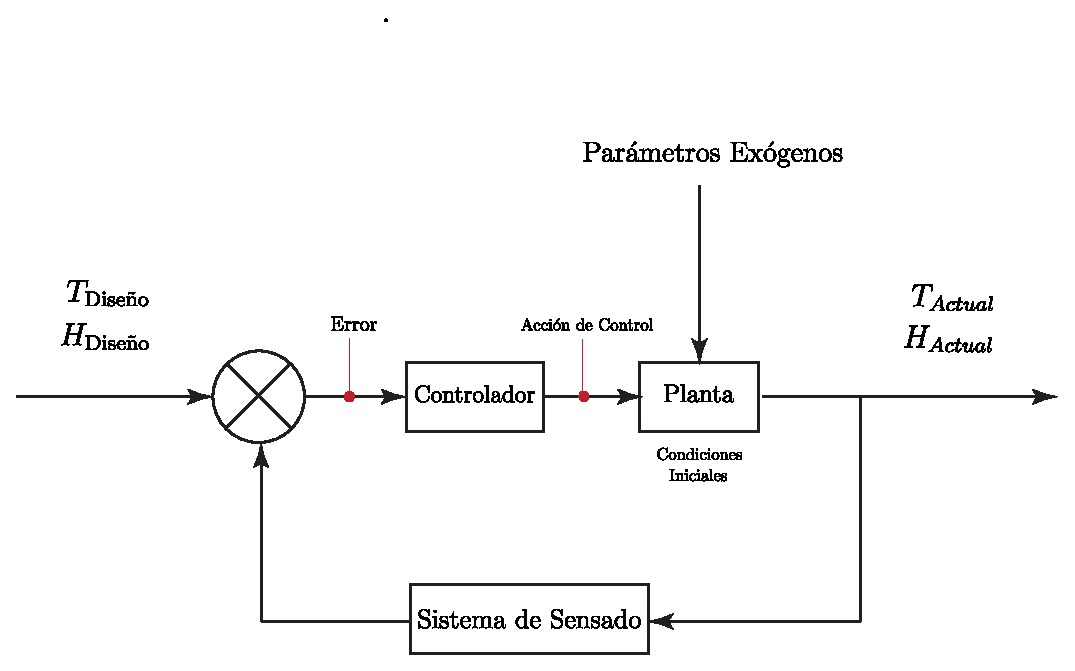
\includegraphics[width=0.90\textwidth]{diagrama_bloques.eps}
    \caption{Diagrama de bloques para el sistema de control cerrado propuesto, para un secador solar de café.}
    \label{fig:diagrama_bloques}
\end{figure}


Un problema clave aún es garantizar una controlabilidad óptima del secado mediante el uso de la menor cantidad posible de parámetros de control. Esto tiene el propósito de reducir la inversión inicial por parte de los caficultores, haciendo que la tecnología sea más accesible y eficiente. Al minimizar los costos sin sacrificar la precisión en el control de la temperatura y la humedad, se puede mejorar la viabilidad económica del sistema, manteniendo la calidad del café durante el proceso de secado.\\


El control preciso de la temperatura y la humedad dentro del secador solar es fundamental para asegurar un secado uniforme y eficiente del grano de café. Esto implica implementar un sistema de control automático que ajuste las condiciones internas basándose en las distribuciones de humedad y temperatura medida en tiempo real. Un control efectivo minimiza el riesgo de sobrecalentamiento o secado desigual, que podría comprometer la calidad del grano. La automatización también permite reaccionar ante variaciones en las condiciones climáticas externas, garantizando que el proceso de secado se mantenga dentro de los parámetros óptimos establecidos.\\


%\subsection{Ventilación forzada y almacenamiento térmico}
%\subsection{Gap: Factibilidad de controladores automáticos}

\section{Análisis Comparativo de Estudios}
La presente sección realiza un análisis comparativo de diversos estudios recientes relacionados con el diseño y desempeño de secadores solares, enfatizando cómo las diferentes configuraciones geométricas, materiales y métodos de modelado impactan la eficiencia térmica y los tiempos de secado. Este examen crítico permite identificar tendencias, avances y brechas en la literatura, estableciendo un marco sólido para fundamentar el desarrollo y optimización de sistemas de secado solar de café.



%\section*{5. Comparación entre estudios}
%\begin{itemize}
%  \item Validaciones mediante OpenFOAM y ANSYS Fluent.
  %\item Métodos de radiación: fvDOM, DO.
 % \item Evaluaciones estadísticas: MAE, %RMSE, R$^2$.
  %\item Influencia de materiales de recubrimiento y pantallas porosas.
%\end{itemize}

\subsection{Resumen de investigaciones recientes}
En diversos estudios se ha demostrado que la geometría y el diseño del secador solar influyen significativamente en la eficiencia térmica y en los tiempos de secado. Por ejemplo, Srichat et al. \cite{Srichat2019} compararon un secador solar con superficie sinusoidal frente a un secador parabólico, encontrando que el primero alcanza temperaturas promedio superiores durante el proceso de secado bajo condiciones equivalentes. Este incremento térmico se traduce en un periodo de secado más corto para el secador sinusoidal, reflejando así una mayor eficiencia energética y mejor aprovechamiento de la radiación solar.\\

Los autores destacan que el secado solar es una técnica efectiva para reducir el contenido de humedad en materiales agrícolas, y que el proceso está condicionado por mecanismos de convección, tanto natural como forzada. En su estudio, describen que los secadores solares consisten en estructuras cerradas con paredes transparentes y techos de polietileno que permiten la entrada de radiación solar y facilitan la remoción de humedad mediante circulación de aire. Las temperaturas internas observadas oscilan entre 35 °C y 65 °C, siendo esta variabilidad clave para el desempeño del secador. El diseño planteado por los investigadores se centró en maximizar el área efectiva expuesta a la radiación solar, manteniendo constantes el volumen y la superficie del secador para asegurar una comparación equitativa. Utilizando modelos genéricos de simulación térmica basados en ANSYS, concluyeron que la configuración sinusoidal alcanzó temperaturas internas más elevadas que la parabólica, confirmando la ventaja del primer diseño.\\

\clearpage

Por otro lado, Chauhan \cite{Chauhan2018} evaluó experimentalmente el desempeño de un secador solar con una pared norte aislada y equipado con un colector de aire caliente ubicado a nivel del suelo, empleando convección natural para optimizar la transferencia térmica. El objetivo principal fue maximizar la eficiencia de conversión de energía solar en calor útil, así como minimizar las pérdidas térmicas por conducción hacia el piso. Los resultados experimentales revelaron que el sistema con colector de aire caliente presentó un coeficiente de desempeño máximo de 0.9, superior al 0.86 registrado en el sistema sin colector. Además, el secador con pared aislada y colector solar evidenció diferencias de temperatura máximas de 30 °C, 28 °C y 18 °C en distintos días de medición, lo que refleja un mejor control térmico y una mayor capacidad para mantener temperaturas óptimas durante el proceso de secado.


\subsection{Innovaciones tecnológicas}
Los secadores solares representan uno de los sectores de mayor demanda energética, dado que requieren un control riguroso del ambiente interior para garantizar el crecimiento óptimo de las plantas y la productividad de los cultivos \cite{Nishad2022}. En este contexto, el almacenamiento de energía térmica mediante materiales de cambio de fase (PCMs, por sus siglas en inglés) surge como una solución innovadora para lograr importantes ahorros energéticos en sistemas de calefacción y refrigeración de invernaderos.\\


Varios investigadores han trabajado en distintas iniciativas que involucran secadores solares para mejorar la eficiencia y desempeño del proceso de secado \cite{Tiwari2018}. Alguna de las mejoras recientes incluyen la incorporacion de colectores termicos solares, materiales de almacenamiento termico como PCM (Phase change materials)\cite{Tiwari2016b}, rock beds y pisos de concreto metalico, inclusive la integracion de bombas de calor. \\


Recientes avances tecnológicos han demostrado que la integración de PCMs en invernaderos permite almacenar el exceso de calor generado por sistemas de climatización activos o pasivos, tales como calefactores, bombas de calor, colectores solares térmicos o muros norte de invernaderos. Además, los PCMs instalados dentro de la estructura del invernadero pueden aportar refrigeración pasiva durante el día, al absorber el exceso de radiación solar, y calefacción pasiva nocturna, liberando el calor acumulado.\\

Diversos estudios señalan que los sistemas con PCMs logran reducir la temperatura diurna hasta en 7°C y aumentarla durante la noche hasta en 9°C respecto a la temperatura ambiente, llegando a cubrir hasta el 30\% de la demanda de calefacción del invernadero. Aunque los costos iniciales de instalación son relativamente altos, estos se compensan con menores gastos de mantenimiento y la reducción del impacto ambiental asociado al uso de combustibles fósiles. Para maximizar la eficiencia energética y económica, es imprescindible definir parámetros de diseño adecuados que consideren las condiciones climáticas locales y los requerimientos específicos de control ambiental.


%\subsection{Gap: Adaptación tecnológica para Panamá}

\section{Criterios de Diseño Recomendados}



La geometría del invernadero debe ser diseñada para maximizar la captación de luz solar y facilitar un flujo de aire adecuado \cite{martinez_estrada_solar_2004}. Esto incluye la orientación, el ángulo de inclinación del techo y el uso de aberturas de ventilación estratégicamente ubicadas. La ventilación cruzada es crucial, ya que permite la extracción efectiva del vapor de agua del grano, lo que mejora la eficiencia del secado. Un diseño geométrico que promueva la circulación del aire garantiza que todas las áreas del grano se expongan a condiciones similares, promoviendo un secado homogéneo.\\

A partir de diversas investigaciones empíricas y recomendaciones presentes en la literatura especializada, se han identificado ciertos parámetros clave para el diseño óptimo de secadores solares. Entre estos destacan:\\


\begin{itemize}
  \item Orientación al sur.
  \item Altura del lecho de secado: 70 cm sobre el suelo.
  \item Material del techo: policarbonato UV.
  \item Inclusión de almacenamiento térmico y ventilación forzada.
\end{itemize}


\subsection{Buenas prácticas de diseño geométrico}

Para maximizar la eficiencia y funcionalidad de un secador solar, es fundamental seguir ciertos criterios de diseño geométrico que optimicen la circulación del aire, la captación solar y la protección del producto. Entre las prácticas recomendadas destacan las siguientes:

\begin{itemize}
\item El café debe colocarse a una altura aproximada de 70 cm sobre el nivel del piso, lo cual facilita una mejor circulación del aire y el proceso de recolección, además de prevenir la absorción de humedad desde el suelo.
\item La orientación del secador solar debe ser preferentemente hacia el sur, con el objetivo de maximizar la exposición a la radiación solar durante su trayectoria diaria.
\item Se debe asegurar que el diseño y la ubicación del secador eviten la generación de sombras que puedan impedir que los rayos solares incidan directamente sobre la superficie del secador durante las horas críticas del día.
\end{itemize}

\subsection{Orientación y disposición}
La orientación y la disposición geométrica de los secadores solares constituyen factores determinantes para optimizar la captación de energía solar, mejorar la distribución térmica interna y reducir pérdidas energéticas. Diversos autores han abordado este aspecto desde enfoques experimentales y analíticos, resaltando su influencia directa en la eficiencia global del proceso de secado.\\

Por ejemplo, Demissie et al.~\cite{Demissie2024} diseñaron y evaluaron un secador solar tipo invernadero semi-cilíndrico, operando dentro de un rango de temperaturas de 40° a 70°C. Este modelo incorporó un modo de secado por convección natural, utilizando materiales como plexiglás y cubiertas de vidrio para maximizar la transmisión de radiación solar y mejorar la retención térmica. Además del análisis técnico, los autores realizaron una evaluación económica comparativa frente a métodos convencionales como el secado a cielo abierto y secadores eléctricos, determinando que el periodo de retorno de la inversión oscila entre 1.5 y 2.1 años, lo que evidencia la viabilidad financiera de la tecnología propuesta.\\

Complementando esta línea de investigación, Mobtaker examinó de forma específica cómo distintas orientaciones, formas y dimensiones de los secadores solares afectan su desempeño térmico y energético. Sus resultados muestran que, en comparación con otras configuraciones, un secador de tipo single span orientado en sentido Este-Oeste puede recibir hasta un 8\% más de radiación solar acumulada a lo largo del año, optimizando así la eficiencia del proceso de secado, especialmente en regiones con variabilidad estacional de la trayectoria solar. Asimismo, el estudio destaca que la implementación de una barrera de ladrillo en el lado norte del secador actúa como aislamiento térmico pasivo, reduciendo significativamente la pérdida de calor por radiación hacia áreas no expuestas al sol y contribuyendo a mantener temperaturas internas más estables.\\

En conjunto, estos hallazgos subrayan la importancia de considerar cuidadosamente la orientación, la forma y los elementos constructivos complementarios durante la etapa de diseño, a fin de maximizar la captación solar y garantizar un secado eficiente y económicamente rentable.



\subsection{Selección de materiales}
De la interacción entre la base y el recubrimiento superior, efectuado en la sección \ref{subsec:buoyancia_y_flujo_de_aire}, se desprende que la selección de materiales debe considerar cuidadosamente sus propiedades térmicas y su disposición estructural para mantener un gradiente favorable que estimule la circulación convectiva natural.\\

En primer lugar, el material de la base del secador debe poseer una alta absorptividad solar y una conductividad térmica moderada, de modo que facilite la acumulación y transmisión uniforme del calor hacia la capa de aire inferior. Materiales como láminas metálicas pintadas de negro mate o superficies con recubrimientos selectivos térmicos pueden incrementar la absorción de radiación solar, generando una base más caliente ($T_\text{base}$) que actúe como fuente estable de calor para inducir la flotación ascendente del aire.\\

Por otro lado, el recubrimiento superior debe optimizar la transmisión de radiación solar y, a la vez, mantener una conductividad térmica relativamente baja, de forma que minimice pérdidas de calor hacia el exterior y permita sostener una diferencia de temperatura que favorezca la convección. Para este fin, materiales como policarbonato alveolar, láminas de polietileno de alta transparencia o vidrio con recubrimientos de baja emisividad resultan adecuados, pues combinan alta transmitancia con capacidad aislante. La incorporación de cámaras de aire o sistemas multicapa en el recubrimiento también contribuye a reducir la transferencia de calor no deseada, reforzando la estratificación térmica positiva.\\

Finalmente, la compatibilidad estructural, la resistencia a la radiación UV y la durabilidad frente a la intemperie son criterios complementarios que deben ser evaluados para garantizar que tanto la base como el recubrimiento mantengan sus propiedades térmicas a lo largo de la vida útil del secador. Esta integración material-geometría-operación resulta clave para asegurar que el gradiente térmico ($T_\text{base} > T_\text{recubrimiento}$) se mantenga en condiciones reales de operación, potenciando la eficiencia del secado mediante un flujo convectivo natural estable y continuo.




%\subsection{Lineamientos preliminares}

\section{Gaps y Oportunidades de Investigación}
\subsection{Lagunas identificadas}

Actualmente existe una falta de algoritmos robustos que combinen de forma realista la absorción, reflexión y transmisión espectral dependiente de la longitud de onda, especialmente relevantes para muros y techos semi-transparentes de secadores solares tropicales. Este vacío limita la precisión de los modelos numéricos, ya que no se cuenta con suficiente validación experimental a escala real para escenarios climáticos altamente variables.\\

Por otro lado, la mayoría de investigaciones aborda la transferencia de calor y masa de manera simplificada, sin acoplar de forma dinámica el microclima interior-exterior. La influencia de la humedad ambiente, la condensación en puntos críticos y su efecto directo sobre la eficiencia del secado siguen siendo poco explorados, dejando espacio para mejoras significativas en la predicción del comportamiento real del sistema.\\

Además, persiste una escasa aplicación de métodos avanzados como la Simulación Directa de Turbulencia (DNS) o LES para captar la estructura fina del flujo en cavidades reducidas. Tampoco se integran de forma transversal análisis CFD con estudios económicos multicriterio ni modelos de control adaptativo de bajo costo que puedan optimizar el consumo energético y garantizar la calidad final del café a partir de la cinética de secado real.


\subsection{Propuestas de acciones futuras}

Estas lagunas abren la posibilidad de desarrollar frameworks de simulación que combinen CFD con algoritmos de Inteligencia Artificial, capaces de ajustar parámetros operativos en tiempo real basándose en datos climáticos locales. Esto permitiría a los productores responder dinámicamente a la variabilidad diaria de radiación y humedad, maximizando la eficiencia sin infraestructura costosa.\\

Otra oportunidad clave es la exploración paramétrica de geometrías optimizadas, utilizando análisis numéricos para comparar formas parabólicas, sinusoidales o cubiertas multi-capa que potencien la captación solar y la circulación natural del flujo de aire. Esta línea puede derivar en prototipos de secadores más eficientes, adaptados a distintas zonas climáticas.\\

Finalmente, la validación de estos modelos debe trascender simulaciones de laboratorio y pruebas puntuales. Implementar series de datos reales mediante sensores IoT y ensayos piloto en fincas permitirá cerrar el ciclo de retroalimentación entre teoría y práctica, asegurando que los desarrollos tecnológicos respondan a las condiciones reales de operación y aporten soluciones escalables para comunidades productoras.




\subsection{Proyectos piloto recomendados}


La incorporación de un sistema de monitoreo continuo de temperatura y humedad internas resulta fundamental para habilitar ajustes dinámicos en tiempo real, asegurando la optimización constante del proceso de secado. Adicionalmente, la implementación de sensores distribuidos que permitan la adquisición de datos en forma continua no solo provee información crítica para la supervisión operativa, sino que también contribuye a la base de datos experimental necesaria para la calibración y validación de los modelos de simulación numérica empleados en el diseño y la posterior optimización del sistema.\\

En la siguiente etapa de la investigación se desarrollará un sistema híbrido que combine simulación CFD de alta fidelidad, mediante OpenFOAM, con redes neuronales informadas por la física (PINNs) para modelar, generalizar y optimizar el funcionamiento de secadores solares de café. Para ello, se generará un conjunto amplio de escenarios CFD variando parámetros de diseño, condiciones climáticas y operativas, capturando la dinámica de transporte de calor y masa. Estos datos alimentarán el entrenamiento de un modelo PINN que incorporará las ecuaciones fundamentales de transferencia de calor, humedad y flujo de aire, permitiendo extrapolar resultados más allá de los casos puntuales y así identificar patrones operativos robustos aplicables a distintos diseños y condiciones externas.\\

Este modelo PINN, una vez validado con datos experimentales provenientes de sensores instalados en los prototipos de secadores, funcionará como modelo sustituto de la simulación CFD para predicciones rápidas en operación real, habilitando estrategias de control predictivo y optimización en línea de temperatura y humedad. Las simulaciones CFD se mantendrán de forma programada y offline como gemelo digital de alta fidelidad, sirviendo para recalibrar periódicamente el modelo de IA ante cambios estructurales o condiciones imprevistas. De este modo, la segunda etapa de la investigación garantizará una arquitectura híbrida que combine coherencia física, capacidad de generalización y velocidad computacional, contribuyendo a un secado homogéneo, reducción de pérdidas de calidad y mayor eficiencia energética en sistemas de secado solar de café.


\clearpage

\section{Conclusiones}
El diseño y funcionamiento eficiente de un secador solar de café exige una integración precisa entre geometría optimizada, gestión térmica pasiva y adaptación a condiciones climáticas variables. Los elementos clave incluyen una configuración estructural que maximice la relación superficie/volumen para mejorar la captación solar sin comprometer la homogeneidad térmica, materiales con propiedades ópticas y térmicas adecuadas para promover el gradiente de temperatura necesario para la convección natural, y un sistema de ventilación inteligente que favorezca el flujo de aire ascendente y el control de humedad interna. Adicionalmente, el secador debe ser robusto frente a la variabilidad ambiental, modular en su construcción y capaz de operar con mínima intervención externa. Sólo mediante la comprensión conjunta de los fenómenos de transferencia de calor, flujo de aire y respuesta climática, es posible diseñar secadores solares que no solo reduzcan pérdidas por mal secado, sino que además preserven el perfil sensorial del café y mejoren la competitividad del productor en mercados especializados

\clearpage

\bibliography{referencias}



\end{document}
